\section{MCRP Emulation Results}
\label{MCRPemulation}

MCRP is evaluated in the Cooja network emulator.  
Fifteen nodes are emulated for the communications network one LPBR and fourteen forming the tree of sensors.  In addition sixteen emulated nodes are used for interference.  
%TODO how are the nodes distributed.
Interference is generated using the model in~\cite{interferenceModel} using settings based on measurements in~\cite{radio2009}. The model has a clear state and an interfered state.  The rules for transitions between states are given in~\cite{interferenceModel}.  Here we allow four states according to the percentage of time where interfering signals are present: no interference, mild (75\% of the time no interference happens), moderate (50\% no interference) and extreme (25\% of the time no interference happens).  However, channel 26 is kept clear from interference in order to ensure RPL set up is unaffected. 

%In the interference state, the interference node generates packets for a time that is uniformly distributed between $9/16$ seconds and $15/16$ seconds. In the clear state the interferer produces no packets and stays in this state for between $3/4 * \emph{clear\textunderscore time}$ and $5/4 * \emph{clear\textunderscore time}$ where \emph{clear\textunderscore time} refers to the rate of interference (ir). 
%Multiple channels interference is used in the simulation to show the hypothesis that MCRP can help avoid interference. The scenario that is considered is where ContikiMAC with RPL system is subject to interference on its channel after set up has successfully completed so the RPL set up is allowed to complete before interference begins.

%The protocol performance in loss over time in the presence of interference is observed. The level of interference used in term of the \textit{clear\_time} is 100\% for no interference, 75\% for mild, 50\% for moderate and 25\% for extreme interference. The percentage represents the ratio of the time the channel is clear for transmission.
%The interference channels are randomly chosen from the available 16 channels.

The emulation has the following phases:
\begin{enumerate}
\item 0-5 minutes -- set up phase with no interference (this prevents RPL failing to build an initial tree in high interference situations).
\item 5-30 minutes -- interference nodes are switched on.  The MCRP tree building and reconfiguration begins.
\item 30-60 minutes -- interference continues and nodes attempt to send data every 30--60 seconds.  The rate of successful transmission is measured.
\end{enumerate}
Measurement of losses in the tree building phase is not made since this phase would be an unrepresentative one off set up cost for any protocol.  It is performance in the steady state that is important since this should last for weeks or years rather than tens of minutes.

The performance of MCRP is compared against the standard ContikiMAC with RPL and Orchestra to demonstrates MCRP abilities in dealing with external and intra interferences. 
%Orchestra does not support RPL downwards routing due to limited memory in TelosB. It however, support the upwards traffic which is require in the experiments as all traffics are directed upwards towards the LPBR.
MCRP is analysed using an end-to-end packet delivery performance metric, setup overhead, channel switching and reconnection delay in MCRP. The transmission success rate is calculated from the sender to the receiver over multiple hops. 
The simulations are repeated ten times. In all plots, the mean value of the ten simulations is plotted with error bars corresponding to one standard deviation in either deviation to give a measure of repeatability. The plots are of the proportion of received packets (from 0\% to 100\%) against time where the loss is measured over the previous time period.  The x-value is shifted slightly left and right to prevent error bars overlapping.

\subsection{Packet Loss Rates}

%\begin{figure}
%\centering
%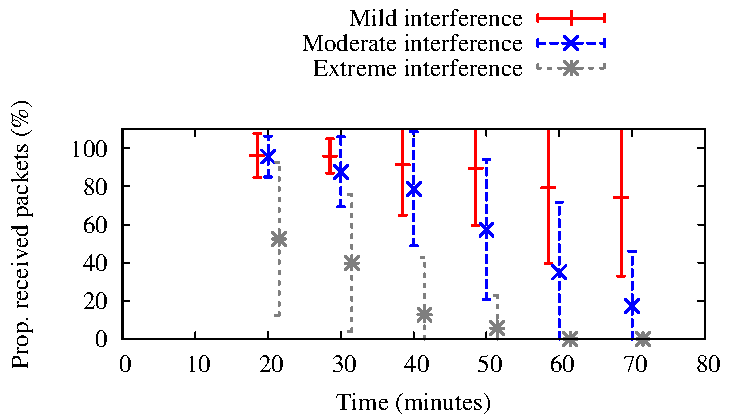
\includegraphics[width=0.45\textwidth]{figures/single_channel.pdf}
%\caption{Emulation: Level of packet loss for mild, moderate and extreme interference levels using single channel}
%\label{fig:interference}
%\end{figure}

%Figure \ref{fig:interference} shows the results in emulation for the single channel RPL protocol. This can be taken as a baseline for improvement for any multi-channel system.  It can be seen that as the emulation proceeds the proportion of received packets falls off.  The network 

Packet loss emulation results for interference on a single channel RPL system can be found in~\cite{mcrp}. These show that when interference is introduced to single channel RPL then the packet loss rate climbs quickly.  In the extreme interference case packet loss had climbed to 100\% by the end of the emulated period. For moderate interference this was 90\%.  For mild interference the figure was only 20\% but the variance was high.  These should be kept in mind as the levels a multiple channel system should improve upon.

\begin{figure}
\centering
\subfigure[Fixed layout]
{\label{fig:randomInterference}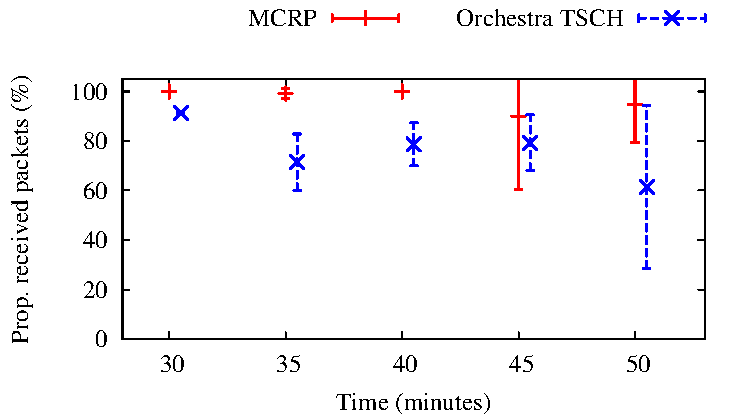
\includegraphics[width=0.45\textwidth]{figures/ri.pdf}}
\subfigure[Random layout]
{\label{fig:randomAll}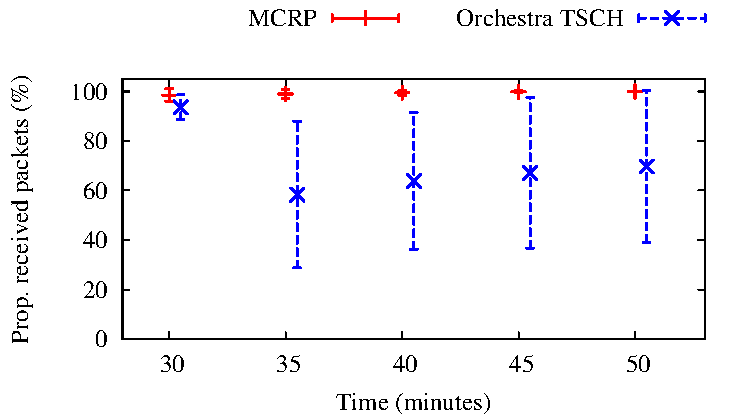
\includegraphics[width=0.45\textwidth]{figures/ra.pdf}}
\caption{Emulation: Level of packet loss for MCRP and Orchestra}
\label{fig:layouts}
\end{figure}


To evaluate MCRP capabilities to cope with interference from many sources, thus channels, and to compare to an existing multichannel protocol Orchestra, the emulations were run where (i) the layout is fixed while the interference channels are chosen by random and (ii) all the nodes including the interference nodes are placed randomly in an area of $150m^2$.  In the fixed layout nodes were positioned in order that the fourteen nodes formed a tree where the LPBR has two children and each of those children has two children (four grand children) and each of those has two children (eight great grand children).
In the experiments, Orchestra uses channel hopping on all 16 channels.  Interference is chosen randomly for the 16 channels so that 4 experience each of the interference conditions: no interference, mild interference, medium interfernce and extreme interference.


Figure \ref{fig:layouts} show MCRP and Orchestra results for the fixed and random nodes layouts.  In these graphs (and all graphs in this paper, x-axis values are shifted slightly to avoid error bars overlaying).
MCRP performs extremely well in both scenarios as the average packet reception rates are between 90\%-100\% and the protocol successfully detects the channels with interference.
Orchestra has higher packet loss compared to MCRP, showing a maximum of 40\% packet loss on average as the channels with interference are being used for transmission periodically. 
In comparison, MCRP selects certain channels to change into after checking the channels condition which gives MCRP a smaller number of packet loss.
MCRP avoids the interference channel while Orchestra hops to the next channel in the next iteration for transmission.

\subsection{Overheads of multiple channel protocols}

Changing channels and probing channels requires signalling overhead for set up.  Extra messages need to be passed for probing and to change channels.  Estimations for setup overhead are given in ~\cite{mcrp}.  Default RPL on ContikiMAC for the topology considered in these experiments completed its set up using 276 packets. MCRP, the multi-channel protocol completed its set up in 716 packets, that is an overhead of 440 packets on top of RPL.  However, it is worth mentioning that this is a one-off cost representing (in this set up) approximately one hour of extra packets where the sensor network deployment would be expected to be in place for weeks, months or longer.  The set up time is 1154 seconds longer for MCRP than RPL.

%Each node has different listening and transmitting channels. When the node is awake, it waits for incoming packets on its listening channel. If the node has a packet to send, it will switch to the next hop listening channel based on the channel information from the neighbour table. The channel switching takes at most 100$\mu$ to switch to the transmission channel. This delay is negligible in the low packet rate WSN. MCRP ContikiMAC uses a transmission phase-lock where the transmission node knows the receiver wake up phase. The node starts transmitting just before the receiver is expected to be awake. The channel switching happens shortly before the receiver is ready to receive the packets, thus the time taken in channel switching does not affect the packet reception.
%The node goes back to sleep once the transmission has succeeded or reached the maximum number of retransmissions (packet loss). In the next iteration, the node is reset and wakes up on its listening channel. 

%The channel reset is done in these cases: (i) the queue buffer is empty, (ii) before sending the next packet from the queue buffer, and (iii) the last packet in the queue buffer has been sent. This reset is done to avoid any delay in packet reception that could happen when the node is awake.2


MCRP also has overhead compared to RPL in terms of reconnection time.  MCRP nodes that disconnect must probe multiple channels to reconnect to the network (as described in section \ref{sec:switching}).  This is obviously slower than RPL that only need probe a single channel.  To test this in isolation we deliberately disconnected a network in the absence of interference by disabling a parent node and measuring the effect on packet transmission.

In the Figure~\ref{fig:reconnectionLayout} node 3 is disabled.
Node 6 and 7 route through node 3 to the LPBR. Nodes 6 and 7 must reconnect through node 5 as shown in Figure \ref{fig:r2}. 

\begin{figure}
\centering
\subfigure[Initial tree]{\label{fig:r1}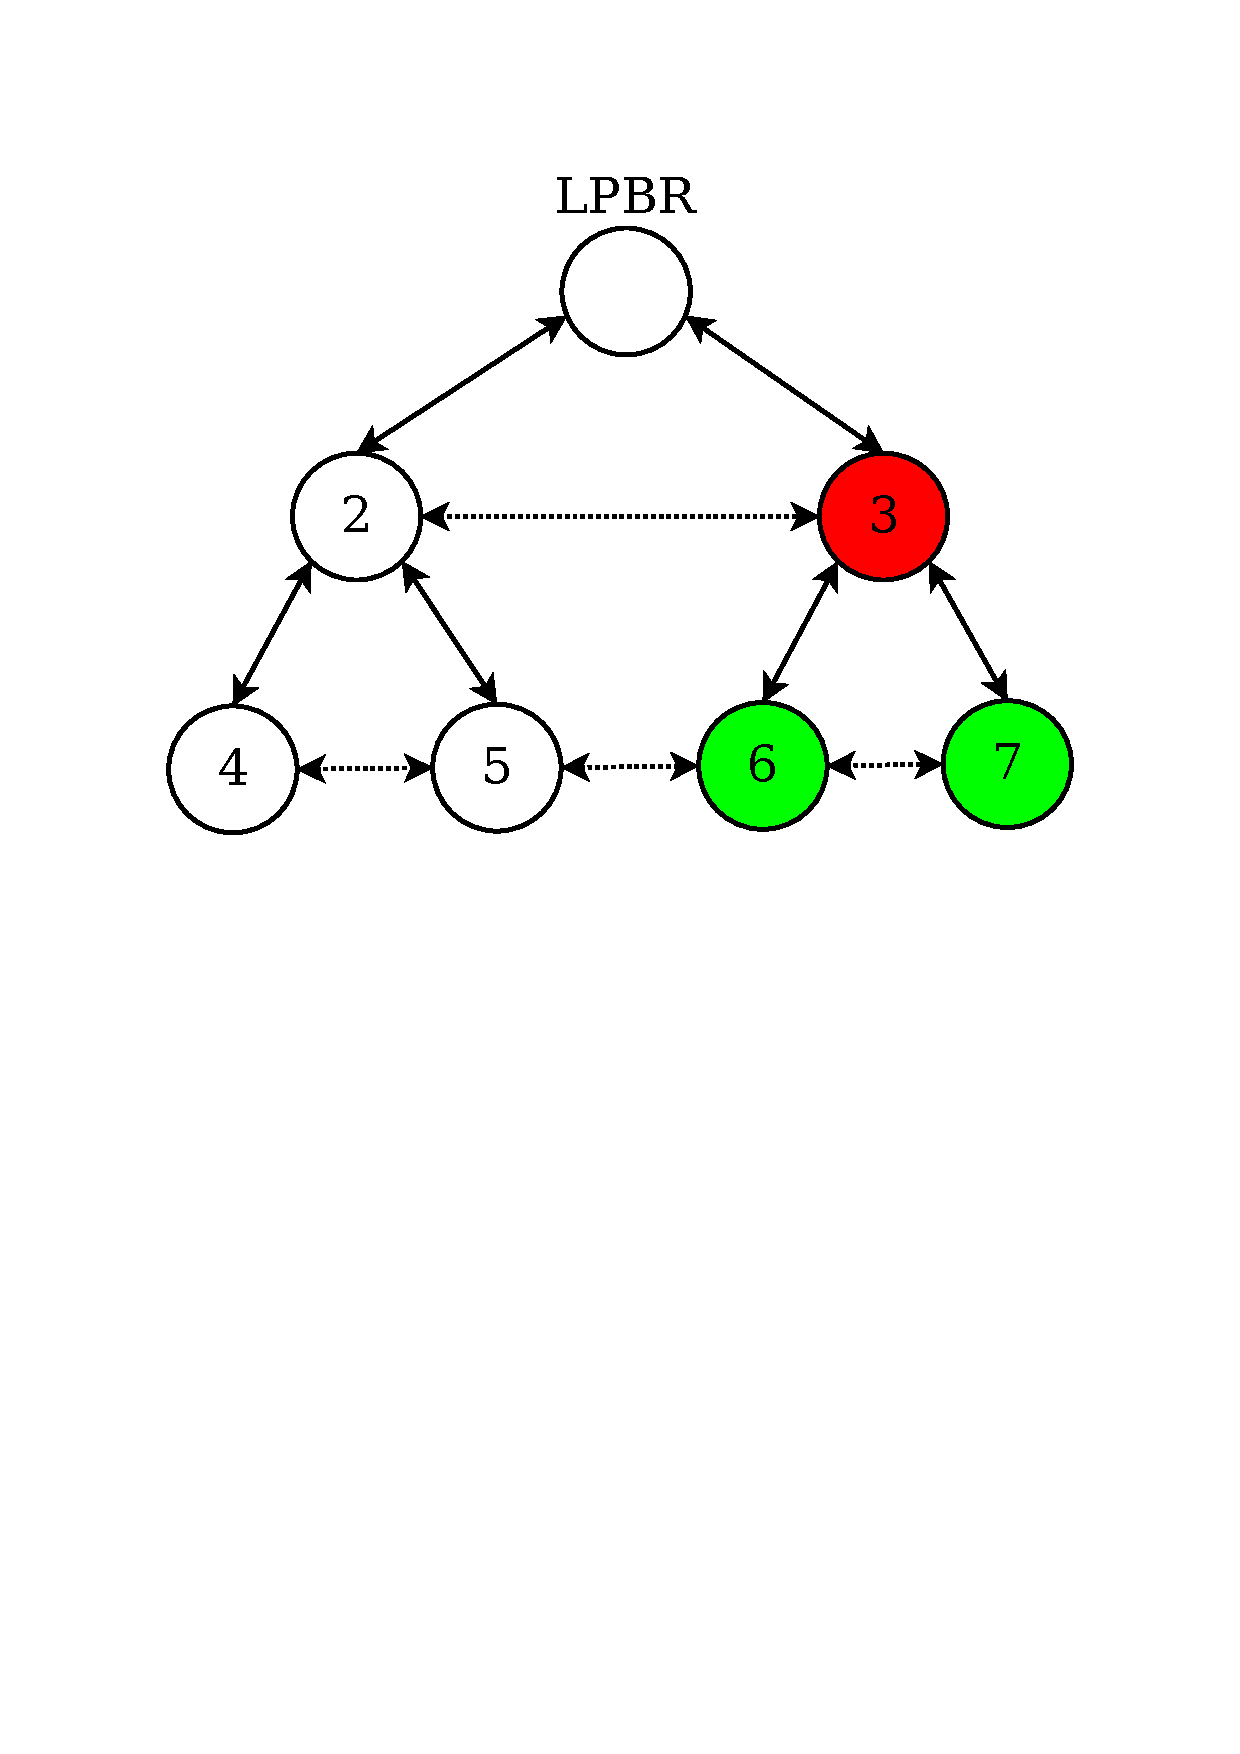
\includegraphics[trim=2cm 16cm 2cm 2cm, clip=true, totalheight=0.12\textheight]
{figures/reconnection1.pdf}}        
\hfill        
\subfigure[Reconstructed tree when node 3 is undetected]{\label{fig:r2}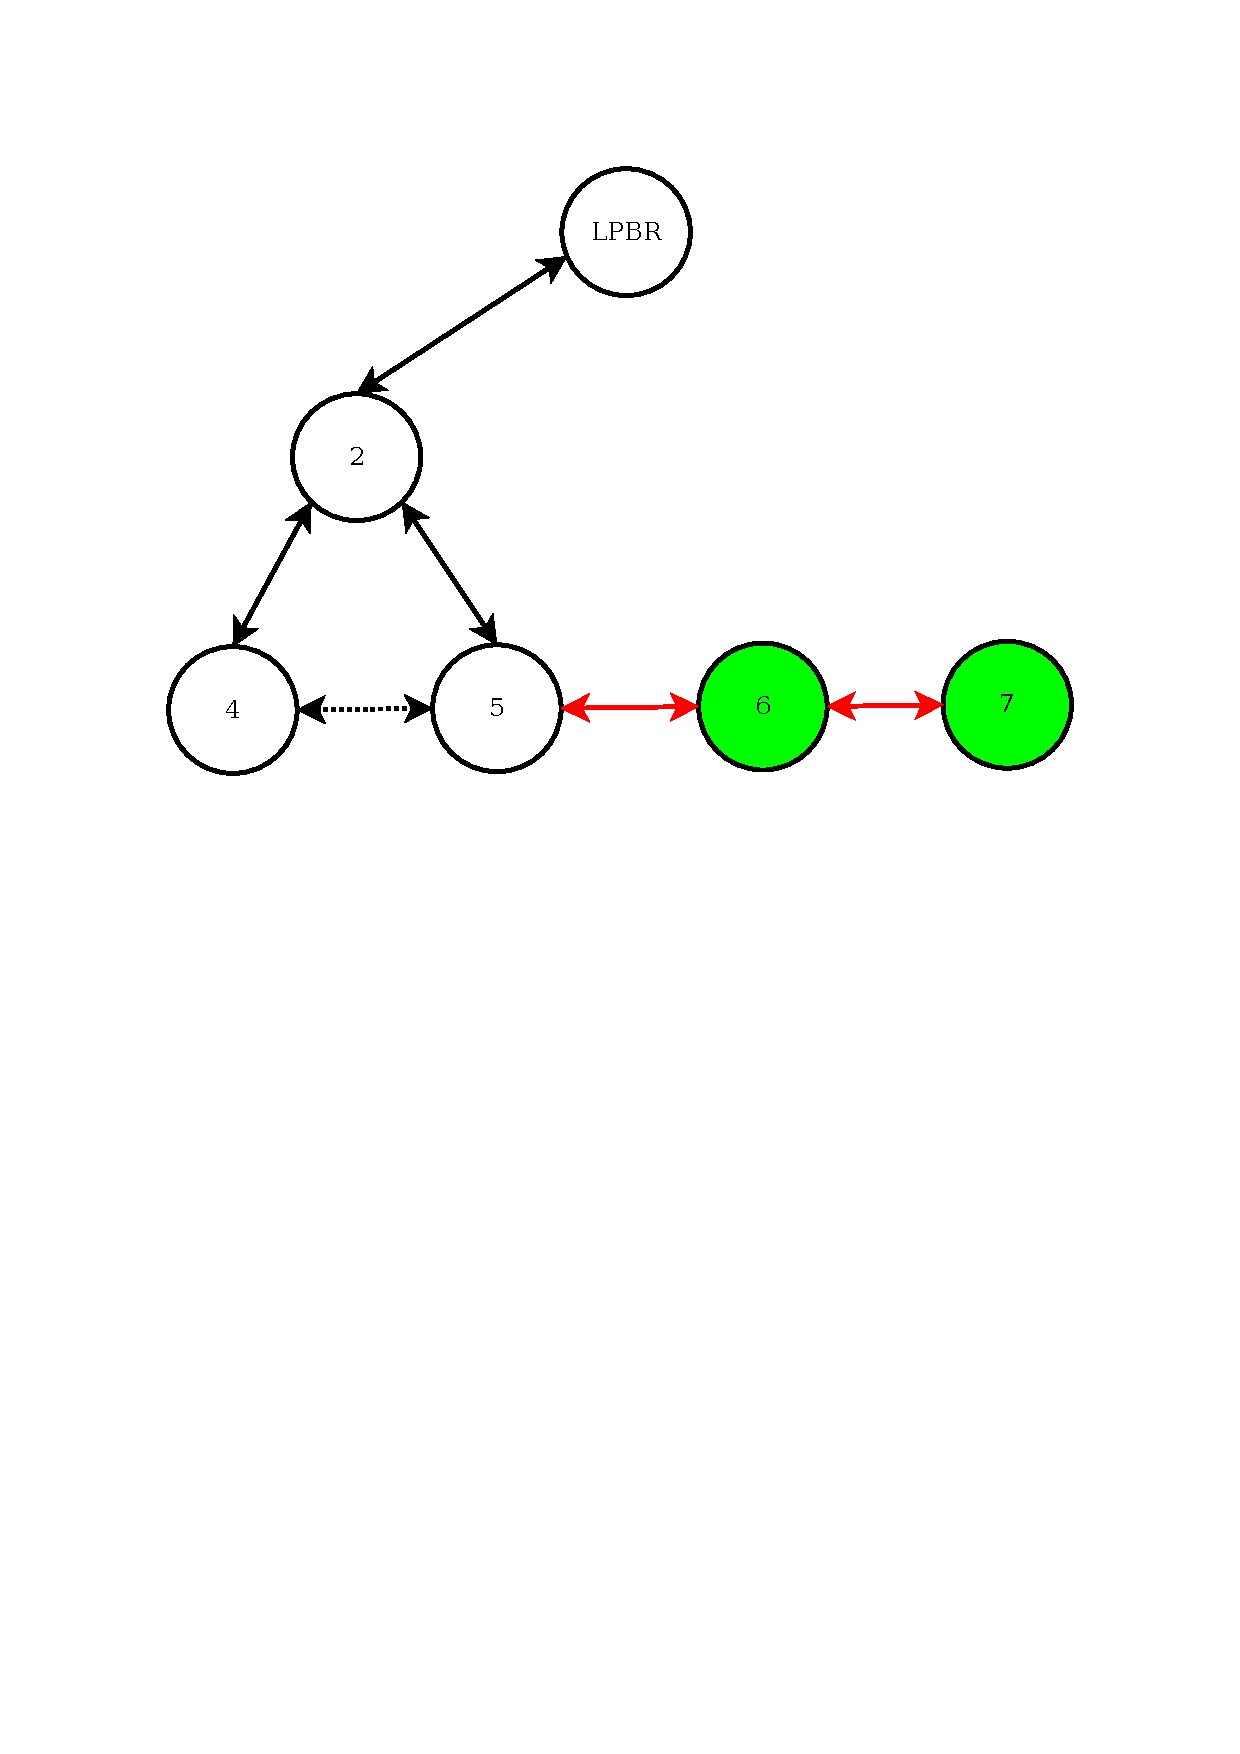
\includegraphics[trim=2cm 16cm 2cm 2cm, clip=true, totalheight=0.12\textheight]
{figures/reconnection2.pdf}}
\caption{A simple tree to emulate the tree reconnection}
\label{fig:reconnectionLayout}
\end{figure}

Figure \ref{fig:reconnection} shows the result of disconnecting node 3 after 54 minutes of emulation.  In MCRP, it took between five and seven minutes before nodes 6 and 7 reconnect.  RPL with single channel is slightly quicker taking three to five minutes. However, considering the more complex task MCRP is performing two minutes added onto reconnection time in the context of a network with low data rates should be acceptable considering the other performance advantages.  In the Orchestra system, by contrast, reconnection is almost instantaneous since the synchronous Orchestra system checks nodes every slot but this is at the expense of greatly increased control traffic.

\begin{figure}
\centering
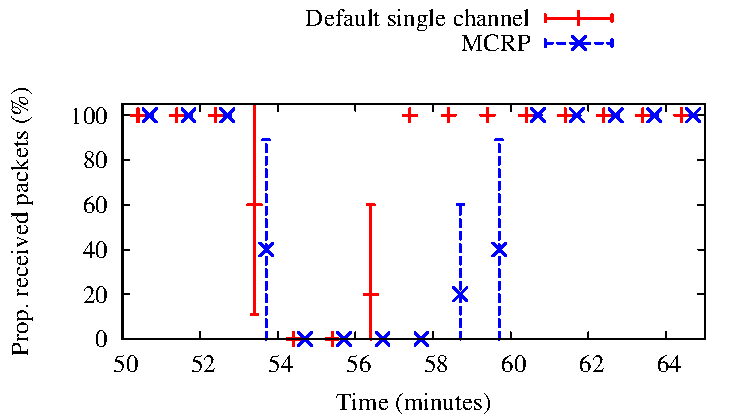
\includegraphics[width=0.45\textwidth]{figures/reconnect.pdf}
\caption{Emulation: Reconnection time taken for MCRP and single channel}
\label{fig:reconnection}
\end{figure}

%Figure \ref{fig:reconnectionLayout} shows the experimental setup to test MCRP reconnection in term of the time taken to detect and adjust the routes when a node fails (run out of battery or cannot be detected). There is no external interference introduced to ensure an accurate convergence time of the topology. The dotted lines represent potential paths and the solid lines are the selected paths. The result from MCRP is compared to a single case scenario with the same setup.


%Comparing to Orchestra, Orchestra is a synchronous protocol. It has a dedicated slot and periodic schedule for RPL signalling which means it detects the failed node quicker unlike in MCRP and default single channel asynchronous protocols. The results from the Orchestra simulation shows that as Orchestra has a slot checking the nodes every minute, it is able to reconnect the nodes without having any packet loss. The disadvantages of Orchestra are, the nodes are listening on the same channel during the broadcast which the known channel is prone to attack. Also, even though Orchestra introduces priority to the traffic, RPL traffic is sent frequently at every period if there is no other higher priority traffic. Trickle timer that is used by the default RPL has the advantage of reducing the number of redundant control packets by doubling the waiting time for the control packets. Orchestra detects failed node quicker at the cost of frequent control packets that are redundant in a stable topology which increases the use of bandwidth and nodes energy consumption.
